% CVPR 2027 submission. Build: tectonic main.tex (from paper/tex)
\documentclass[10pt,twocolumn,letterpaper]{article}

\usepackage[review]{cvpr}
\usepackage[T1]{fontenc}
\usepackage{times}
\usepackage{graphicx}
\usepackage{amsmath,amssymb}
\usepackage{booktabs}
\usepackage{multirow}
\usepackage{xcolor}
\definecolor{cvprblue}{rgb}{0.21,0.49,0.74}
\usepackage{colortbl}
\usepackage{enumitem}
\usepackage{microtype}
\renewcommand{\arraystretch}{0.93}
\setlength{\textfloatsep}{8pt}
\setlength{\abovecaptionskip}{4pt}
\usepackage[pagebackref,breaklinks,colorlinks,citecolor=cvprblue,linkcolor=cvprblue,urlcolor=cvprblue]{hyperref}

\def\confName{CVPR}
\def\confYear{2027}
\def\paperID{XXXX}

\graphicspath{{../figures/}}
\definecolor{tbd}{RGB}{176,96,0}
\definecolor{tbdbg}{RGB}{255,246,230}
\newcommand{\tbd}[1]{\colorbox{tbdbg}{\textcolor{tbd}{\footnotesize pending: #1}}}
\newcommand{\cur}{\textsc{cur}}
\newcommand{\curerr}{\textsc{cur-err}}
\newcommand{\auroc}{\textsc{auroc}}
\newcommand{\absrel}{\textsc{AbsRel}}
\newcommand{\bench}{HalluBench-3D}
\newcommand{\ci}[3]{#1\,{\scriptsize[#2,\,#3]}}

\title{Observe, Imagine, Abstain:\\Hallucination-Aware 3D Reconstruction with Discrete Diffusion and Continual Adaptation}

\author{Anonymous \confName~submission\\Paper ID \paperID}

\begin{document}
\maketitle

\begin{abstract}
Feed-forward 3D foundation models reconstruct a scene from unposed photographs in a single pass. Where no photograph shows a surface, they fill the gap from learned priors, and they often assign the invented geometry a confidence indistinguishable from that of observed geometry. We call this geometric hallucination and define it operationally: a predicted point is hallucinated when it lies on a surface that no input view observes. \bench{} produces such labels for free by hiding a 3D region of the ground-truth surface in every input view, so that every pixel inside the region is unsupported and every pixel far from it is supported. We ask whether a model's native confidence separates the two (\auroc) and how much unsupported geometry survives a threshold that keeps 90\% of supported geometry, the Confident-Unsupported Rate (\cur). Across five models (VGGT, Pi3, Pi3X, MapAnything, Depth Anything 3), 18 DTU scans and 18 CO3Dv2 scenes, with five mask placements, two region sizes and three fills each, native confidence lets between 24\% and 81\% of unsupported pixels through. A realistic inpainted fill makes leakage worse, not better; dropping views or adding a distractor image leaves it unchanged; and the cheapest alternative, variance over perturbed inputs, is worse than native confidence on both backbones we tried. The ranking of models also changes between the lab rig and phone captures: only Pi3 behaves the same on both. We then propose a method that does not forbid imagination but makes it explicit: a frozen backbone with a small discrete diffusion head draws $K$ geometry samples, agreement marks observed geometry, disagreement marks imagined geometry, and the rest abstains. The method and its continual-adaptation variant are specified here; their numbers are pending and marked as such. Code, benchmark and the full run log will be released.
\end{abstract}

%------------------------------------------------------------------------
\section{Introduction}
\label{sec:intro}

\begin{figure*}[t]
\centering
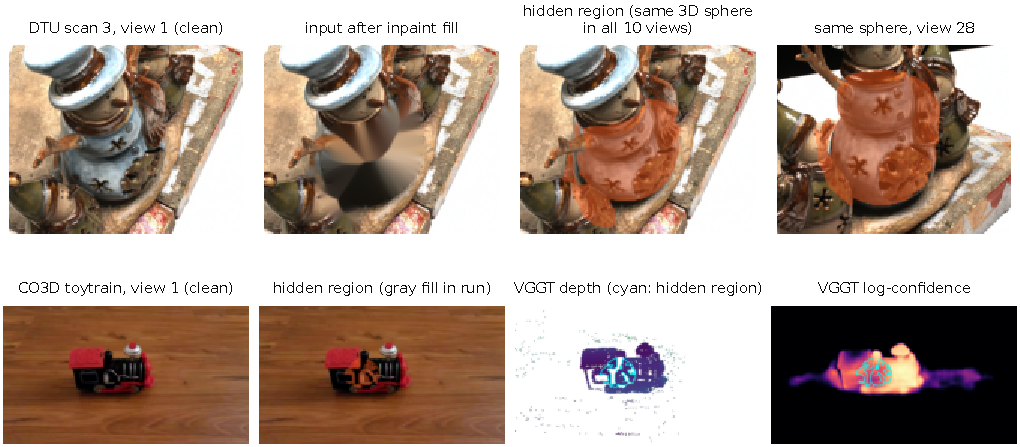
\includegraphics[width=0.84\textwidth]{fig1_teaser}
\caption{\textbf{What a model does with a surface it cannot see.} Top: a DTU scan with one 3D region of the ground-truth surface hidden in all ten input views and inpainted so no seam remains. Bottom: a CO3Dv2 phone capture treated the same way. The top row shows the protocol: the same 3D sphere hides the region in every view, including a view from the other side of the rig. The bottom row shows what the backbone (VGGT) does with it: plausible geometry inside the hidden region, with confidence close to its value outside. The cyan contour marks the unsupported pixels. Model panels are the recorded run outputs.}
\label{fig:teaser}
\end{figure*}

Feed-forward 3D reconstruction has moved from pairwise pointmaps~\cite{dust3r,mast3r} to models that take dozens of unposed images and return dense geometry in one forward pass~\cite{vggt,pi3,mapanything,da3}. These models are trained to output geometry at every pixel, including pixels whose true surface is not visible in any input view. The training objective rewards a plausible guess, so the models learn to guess. The guess is often good, and that is useful. The trouble is that the confidence map, the one signal a user has, does not say which parts were observed and which were guessed.

Suppose you are a conservator looking at a reconstruction of a dome, and you see a crack. Before you send someone up a scaffold, you want to know whether any photograph shows that crack or whether the model drew it from what domes usually look like. Today you cannot tell. The confidence map is bright in both cases.

We make three contributions.

\begin{enumerate}[leftmargin=*,itemsep=1pt,topsep=2pt]
\item \textbf{A definition and a benchmark.} We define hallucinated geometry as predicted points on surfaces that no input view shows. \bench{} produces these labels by 3D-consistent masking of ground-truth surfaces, with controls on the same pixels under clean input. We report \auroc, \cur{} and \curerr{} for five models on DTU and CO3Dv2, three fill types, an inpainted fill, and stress tests (view dropping, low parallax, a distractor image), each with cluster-bootstrap intervals and paired permutation tests.
\item \textbf{A method that separates observed from imagined geometry.} A frozen backbone and frozen language-aligned features feed a uniform-state discrete diffusion head over quantized geometry tokens, trained self-supervised by masking regions and recovering their tokens. At test time $K$ samples give geometry, a three-way label (observed, imagined, abstain), and an uncertainty from sample disagreement.
\item \textbf{Continual adaptation.} Low-rank adapters on the diffusion head with a small replay buffer adapt to a stream of new sites, reported against naive fine-tuning.
\end{enumerate}

Contribution 1 is complete and every number in Sections~\ref{sec:bench} and~\ref{sec:results} comes from a logged run. Contributions 2 and 3 are specified in Section~\ref{sec:method}; their experiments are pending and are marked \tbd{run id} rather than estimated. We would rather show you an honest gap than a filled one. That is, after all, the point of the paper.

The headline claim we test, and do not assume, is that native confidence fails to flag unsupported geometry across current models. It holds, and it holds more strongly on phone captures than on the lab rig.

%------------------------------------------------------------------------
\section{Related work}
\label{sec:related}

\paragraph{Feed-forward 3D reconstruction.}
DUSt3R and MASt3R~\cite{dust3r,mast3r} predict pointmaps for image pairs. VGGT~\cite{vggt}, Pi3 and Pi3X~\cite{pi3}, MapAnything~\cite{mapanything}, VGGT-Omega~\cite{vggtomega} and Depth Anything 3~\cite{da3} extend this to many unposed views in one pass. Each exposes a per-pixel confidence trained as a loss weight on observed data; none is trained to distinguish observed from unobserved surfaces. Pi3X replaces Pi3's near-binary confidence with continuous quality levels, so confidence semantics differ even within one family. MapAnything also offers a multi-view consistency confidence, which we include as a baseline.

\paragraph{Hallucination in feed-forward 3D.}
Bratulic et al.~\cite{bratulic2025} probe DUSt3R, VGGT and DA3 and show that attention heads keep matching correspondences after small patches are occluded, concluding that these models hallucinate missing correspondences from learned priors; they measure attention and Sampson error on ShapeNet pairs, not confidence or 3D labels. Paul et al.~\cite{paul2026} benchmark hallucination at the input level: unrelated scenes, repeated images and noise still produce dense geometry, scored by COLMAP-based consistency. 3D-Mirage~\cite{mirage} studies monocular depth under visual illusions. Our definition is per point, inside a real scene, with exact supported and unsupported labels, and it tests whether native confidence separates them.

\paragraph{Uncertainty for feed-forward 3D.}
ReVar3R~\cite{revar3r} aligns perturbed runs to a common frame and takes per-point variance; it beats native confidence on AUSE in most conditions but, by its authors' account, misses stable systematic bias, which is exactly what a confidently filled region is. Trust3R~\cite{trust3r} fits an evidential head on a frozen backbone. GeoCond~\cite{geocond} adds pose-level uncertainty and a refinement gate. Deng et al.~\cite{deng2026} audit the calibration of seven backbones and find implied uncertainty at least $2.4\times$ too small. All of these score uncertainty against ground-truth error, which conflates confident errors on observed surfaces with confident predictions on surfaces no view saw. \cur{} isolates the second case. Free Geometry~\cite{freegeom} and TTT3R~\cite{ttt3r} adapt at test time, but neither labels unsupported regions.

\paragraph{Generative and multi-sample 3D.}
Z3D~\cite{z3d} decodes hidden surfaces from frozen VGGT features with linear probes and diffusion, evidence that unobserved geometry is present in the features. VolFill~\cite{volfill} reports sample variation about $1.3\times$ larger in occluded regions for single-view amodal reconstruction, the signal we use in the multi-view setting. Diffusion depth ensembles~\cite{marigold,perfectingdepth} give sample-disagreement uncertainty but need scale and shift alignment before variance is taken; we do the same. URSA~\cite{ursa} provides the uniform-state discrete diffusion sampler we build on; we found no prior use of it for 3D.

\paragraph{Hallucination in vision-language models.}
Object hallucination benchmarks such as POPE~\cite{pope} label statements unsupported by the image. Ours is the geometric analogue: geometry unsupported by any view.

%------------------------------------------------------------------------
\section{Defining geometric hallucination}
\label{sec:def}

Given input views $I_1,\dots,I_N$, a model returns for each view $i$ a depth map $D_i$ and a confidence map $C_i$. A pixel $p$ in view $i$ is \emph{supported} if its ground-truth surface point is visible in at least one input view, and \emph{unsupported} if it is visible in none. A model hallucinates at $p$ when it outputs geometry at an unsupported $p$ with high confidence.

\paragraph{Why confidence is the wrong tool.}
Native confidence is trained as a per-pixel loss weight on observed data. It learns to be low where the regression target is noisy (edges, specular surfaces) and high where it is smooth. A region that no view sees and that the prior fills smoothly therefore receives high confidence by construction. Section~\ref{sec:results} measures how large this effect is.

\paragraph{Metrics.} All are computed per (model, scene, seed, radius, fill) and averaged with cluster-bootstrap intervals over scenes.
\begin{itemize}[leftmargin=*,itemsep=1pt,topsep=2pt]
\item \auroc: $P(C_S > C_U)$ with ties counted half. 1.0 means every supported pixel outranks every unsupported one; 0.5 means confidence carries no information about support.
\item \cur: choose $\tau$ so that 90\% of supported pixels have $C\ge\tau$; \cur{} is the fraction of unsupported pixels with $C\ge\tau$. This is the hallucination rate you would experience after filtering by confidence.
\item \curerr: the fraction of unsupported pixels above $\tau$ whose \absrel{} exceeds 0.1. Confident and wrong.
\item $\absrel_U$, $\absrel_S$: depth error on unsupported and supported pixels after median scaling fitted on supported pixels only.
\item Controls: the same pixels under clean input ($\absrel_U$ ctrl, \auroc{} ctrl) and the ratio of median confidence inside the hidden region to its clean value.
\end{itemize}

%------------------------------------------------------------------------
\section{\bench}
\label{sec:bench}

\begin{figure*}[t]
\centering
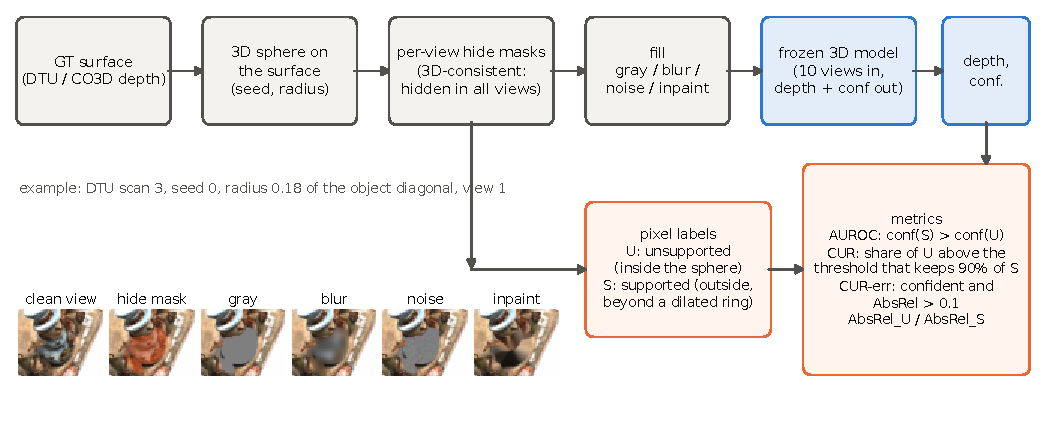
\includegraphics[width=0.8\textwidth]{fig2_pipeline}
\caption{\textbf{The benchmark protocol.} A sphere is placed on the ground-truth surface; every pixel in every view whose ground-truth point falls inside it is hidden, so the hidden region is 3D-consistent. Hidden pixels are filled (gray, blur, noise or inpaint), the model runs on the filled views, and its depth and confidence are scored against the unsupported (U), supported (S) and ring labels. The same pixels are also scored under clean input as a control.}
\label{fig:pipeline}
\end{figure*}

\paragraph{Protocol.}
For each scene we take 10 views. A sphere is centred on a random ground-truth surface point in the reference view, with radius 0.10 or 0.18 of the object's bounding-box diagonal, resampled until it covers 2 to 35\% of the reference view. Every pixel in every view whose ground-truth point lies inside the sphere is hidden (Figure~\ref{fig:pipeline}). Hidden pixels are filled with gray, a blur of the original, uniform noise, or an inpainting of the surround~\cite{telea}; fill type is an ablation so that results are not an artefact of a visible patch. Labels: U is hidden in all views; S is valid and outside a 6-pixel dilation of the hidden region; the ring in between is ignored. Five mask seeds per scene; masks are deterministic in (scene, seed, radius).

\paragraph{Datasets.}
\emph{DTU}~\cite{dtu}: the 18 scans of the MVSNet validation split, 10 views spread over the 49-camera rig, model input $420\times518$. \emph{CO3Dv2}~\cite{co3d}: 18 scenes, the two depth-carrying sequences of each of nine categories (apple, ball, bench, hydrant, mouse, teddybear, toytrain, toytruck, vase) from the single-sequence subset, with the official COLMAP depth as ground truth. The 10 views are spread over the full orbit, so the hidden region is seen from the back as well as the front. Frames are $640\times360$ phone video; models run at $518\times294$ (or the transpose for landscape sequences). Everything else, including every threshold, is unchanged from DTU.

\paragraph{Correctness guards.}
Before any model is scored we check that ground-truth depth reprojects consistently between view pairs and that unsupported points of view $i$, where visible in view $j$, land inside view $j$'s hidden mask. On DTU: reprojection agreement 0.80 to 0.82 at a 1\% depth tolerance and U-transfer 0.96 to 0.99. CO3Dv2 cameras were converted from the PyTorch3D convention and checked by projecting the official point cloud (median depth error 0.7 to 2.5\% per view); with an occlusion-aware 3\% tolerance, reprojection agreement is 0.92 to 1.00 on CO3D and 0.99 on DTU, and U-transfer is 0.90 to 0.98 on 17 of 18 scenes. The eighteenth (a vase with a small hidden sphere near the silhouette) scores 0.80; we keep it and report in Section~\ref{sec:results} that removing it changes nothing.

\paragraph{Pipeline validation.}
On a synthetic DTU-format scene, an oracle that knows what is hidden scores \auroc{} 1.000 and \cur{} 0.000, and a blind guesser with flat confidence scores \auroc{} 0.500 and \cur{} 0.90 (the 10\% of supported pixels dropped by $\tau$ is the expected floor). These numbers validate the code, not any model.

\paragraph{Models.}
VGGT-1B~\cite{vggt} (depth and depth confidence), Pi3 and Pi3X~\cite{pi3} (local point $z$ and sigmoid confidence), MapAnything~\cite{mapanything} (image-only metric mode), and Depth Anything 3~\cite{da3} (Large 1.1). Same views, resolution and fp16 budget for all, on a single T4. VGGT-Omega is gated and not yet run.

\paragraph{Statistics.}
Means carry 95\% cluster-bootstrap intervals over scenes (10,000 resamples; each scene contributes its mean over seeds). Pairwise comparisons use a paired sign-flip permutation test on per-scene means (20,000 permutations), Holm-corrected within each family of pairs.

%------------------------------------------------------------------------
\section{Results on \bench}
\label{sec:results}

\begin{table*}[t]
\centering
\caption{\textbf{DTU, five models, full configuration.} 18 scans $\times$ 5 mask seeds $\times$ 2 radii $\times$ 3 fills, pooled over radii; mean [95\% cluster-bootstrap CI over scans]. \emph{conf ratio} is the median confidence inside the hidden region divided by its value under clean input. Runs P1-full and P2-full, T4, fp16.}
\label{tab:dtu}
\footnotesize
\setlength{\tabcolsep}{4pt}
\begin{tabular}{llcccccc}
\toprule
model & fill & \auroc & \cur & \curerr & $\absrel_U$ & $\absrel_U$ ctrl & conf ratio \\
\midrule
VGGT-1B & gray  & \ci{0.973}{0.955}{0.987} & \ci{0.067}{0.031}{0.111} & 0.000 & 0.018 & 0.006 & 0.051 \\
VGGT-1B & blur  & \ci{0.886}{0.843}{0.922} & \ci{0.263}{0.203}{0.324} & 0.000 & 0.011 & 0.006 & 0.241 \\
VGGT-1B & noise & \ci{0.919}{0.892}{0.945} & \ci{0.222}{0.145}{0.304} & 0.000 & 0.014 & 0.006 & 0.192 \\
Pi3 & gray  & \ci{0.981}{0.972}{0.988} & \ci{0.053}{0.025}{0.085} & 0.001 & 0.020 & 0.014 & 0.057 \\
Pi3 & blur  & \ci{0.923}{0.895}{0.947} & \ci{0.236}{0.156}{0.326} & 0.001 & 0.018 & 0.014 & 0.261 \\
Pi3 & noise & \ci{0.902}{0.865}{0.934} & \ci{0.325}{0.219}{0.438} & 0.002 & 0.020 & 0.014 & 0.411 \\
Pi3X & gray  & \ci{0.940}{0.902}{0.971} & \ci{0.202}{0.085}{0.337} & 0.002 & 0.022 & 0.017 & 0.335 \\
Pi3X & blur  & \ci{0.826}{0.782}{0.865} & \ci{0.512}{0.397}{0.630} & 0.002 & 0.020 & 0.017 & 0.739 \\
Pi3X & noise & \ci{0.801}{0.734}{0.864} & \ci{0.551}{0.390}{0.711} & 0.004 & 0.022 & 0.017 & 1.091 \\
MapAnything & gray  & \ci{0.861}{0.812}{0.905} & \ci{0.374}{0.272}{0.480} & \ci{0.195}{0.125}{0.269} & 0.222 & 0.111 & 0.650 \\
MapAnything & blur  & \ci{0.773}{0.720}{0.825} & \ci{0.580}{0.482}{0.672} & \ci{0.277}{0.197}{0.361} & 0.135 & 0.111 & 0.677 \\
MapAnything & noise & \ci{0.712}{0.645}{0.773} & \ci{0.664}{0.566}{0.758} & \ci{0.295}{0.211}{0.390} & 0.129 & 0.111 & 0.709 \\
Depth Anything 3 & gray  & \ci{0.723}{0.664}{0.780} & \ci{0.703}{0.596}{0.804} & 0.003 & 0.017 & 0.013 & 0.804 \\
Depth Anything 3 & blur  & \ci{0.682}{0.611}{0.744} & \ci{0.711}{0.619}{0.796} & 0.003 & 0.016 & 0.013 & 0.800 \\
Depth Anything 3 & noise & \ci{0.740}{0.686}{0.793} & \ci{0.690}{0.578}{0.793} & 0.001 & 0.017 & 0.013 & 0.855 \\
\bottomrule
\end{tabular}
\end{table*}

\subsection{DTU: native confidence leaks}
\label{sec:dtu}

Table~\ref{tab:dtu} gives the full DTU configuration (the per-run spread is in the supplementary material). Pooled over the two natural-statistics fills (blur and noise), \cur{} is 0.242 for VGGT, 0.281 for Pi3, 0.532 for Pi3X, 0.622 for MapAnything and 0.701 for Depth Anything 3, with \auroc{} 0.903, 0.912, 0.813, 0.743 and 0.711. Three tiers emerge. VGGT and Pi3 drop their confidence inside the hidden region (to 19 to 41\% of its clean value) yet still let one in four unsupported pixels through a threshold that keeps 90\% of supported ones. Pi3X leaks one in two, and under a noise fill it is as confident about geometry it cannot see as about geometry it can (ratio 1.09). MapAnything and Depth Anything 3 are close to blind to non-observation. DA3's confidence inside the hidden region stays at 80 to 86\% of its clean value for every fill, including the gray patch; whatever its confidence encodes, it is not observation.

Pairwise, after Holm correction over the ten pairs: VGGT and Pi3 are indistinguishable ($p=0.41$); both leak less than Pi3X ($p\le0.0015$), MapAnything and DA3 ($p=0.0005$). Pi3X versus DA3 ($p=0.052$), Pi3X versus MapAnything and MapAnything versus DA3 ($p=0.19$) are not separated.

\paragraph{Confident and wrong.}
On DTU the imagined depth is accurate for four of the five models ($\absrel_U$ 0.011 to 0.022, about 1.3 to $2\times$ the clean value), so \curerr{} stays near zero. The failure is that you cannot tell imagined from observed, not that the imagination is poor. MapAnything is the exception: 29\% of its unsupported pixels are confident and wrong by more than 10\% \absrel, on top of a 10\% error on supported pixels in image-only metric mode (unchanged at its native input size).

\paragraph{Gate.}
Before scaling the benchmark we fixed a pass condition: \cur{} above zero with intervals excluding zero, and \auroc{} clearly below one on the natural fills. It passes for all five models. The effect is not an artefact of a gray patch, and it is strongly model dependent.


\subsection{Stress tests: the leak is not a patch artefact}
\label{sec:stress}

\begin{table*}[t]
\centering
\caption{\textbf{Stress tests on DTU.} 18 scans $\times$ 2 mask seeds, radius 0.18, models VGGT, Pi3X, DA3. Reference rows are the matching cells of Table~\ref{tab:dtu} (blur, 10 spread views, seeds 0 and 1). Last column: paired \cur{} difference against the reference with a sign-flip $p$ over scans. Run P2-stress.}
\label{tab:stress}
\footnotesize
\setlength{\tabcolsep}{4pt}
\begin{tabular}{llccccl}
\toprule
model & test & \auroc & \cur & \curerr & $\absrel_U$ & \cur{} vs ref \\
\midrule
VGGT-1B & reference & \ci{0.902}{0.868}{0.930} & \ci{0.259}{0.175}{0.349} & 0.000 & 0.010 & \\
VGGT-1B & inpaint fill & \ci{0.867}{0.821}{0.907} & \ci{0.347}{0.255}{0.443} & 0.001 & 0.018 & $+0.088$ ($p=0.031$) \\
VGGT-1B & 5 views & 0.902 & \ci{0.269}{0.173}{0.377} & 0.000 & 0.011 & $+0.010$ ($p=0.63$) \\
VGGT-1B & 3 views & 0.899 & \ci{0.259}{0.167}{0.361} & 0.000 & 0.013 & $+0.001$ ($p=0.98$) \\
VGGT-1B & low parallax & 0.911 & \ci{0.214}{0.110}{0.334} & 0.000 & 0.021 & $-0.045$ ($p=0.35$) \\
VGGT-1B & + distractor & 0.905 & \ci{0.257}{0.179}{0.340} & 0.000 & 0.011 & $-0.002$ ($p=0.90$) \\
Pi3X & reference & \ci{0.828}{0.781}{0.870} & \ci{0.521}{0.390}{0.650} & 0.002 & 0.024 & \\
Pi3X & inpaint fill & \ci{0.786}{0.731}{0.836} & \ci{0.589}{0.473}{0.702} & 0.004 & 0.022 & $+0.068$ ($p=0.005$) \\
Pi3X & 5 views & 0.822 & \ci{0.539}{0.411}{0.661} & 0.006 & 0.024 & $+0.018$ ($p=0.44$) \\
Pi3X & 3 views & 0.840 & \ci{0.497}{0.373}{0.618} & 0.032 & 0.051 & $-0.024$ ($p=0.64$) \\
Pi3X & low parallax & 0.812 & \ci{0.523}{0.376}{0.671} & 0.040 & 0.050 & $+0.002$ ($p=0.98$) \\
Pi3X & + distractor & 0.829 & \ci{0.510}{0.368}{0.650} & 0.002 & 0.024 & $-0.011$ ($p=0.66$) \\
DA3 & reference & \ci{0.712}{0.632}{0.783} & \ci{0.679}{0.569}{0.791} & 0.006 & 0.018 & \\
DA3 & inpaint fill & 0.726 & \ci{0.688}{0.605}{0.774} & 0.009 & 0.018 & $+0.008$ ($p=0.87$) \\
DA3 & 5 views & 0.697 & \ci{0.785}{0.703}{0.865} & 0.005 & 0.019 & $+0.106$ ($p=0.008$) \\
DA3 & 3 views & 0.729 & \ci{0.667}{0.560}{0.770} & 0.018 & 0.031 & $-0.012$ ($p=0.81$) \\
DA3 & low parallax & \ci{0.863}{0.785}{0.925} & \ci{0.372}{0.230}{0.520} & 0.008 & 0.029 & $-0.307$ ($p=0.0003$) \\
DA3 & + distractor & \ci{0.660}{0.580}{0.734} & \ci{0.775}{0.680}{0.868} & 0.003 & 0.019 & $+0.096$ ($p=0.0004$) \\
\bottomrule
\end{tabular}
\end{table*}

A reasonable objection to Table~\ref{tab:dtu} is that a filled patch is visible, and the model is reacting to the patch rather than to the absence of a surface. Table~\ref{tab:stress} and Figure~\ref{fig:stress} answer it four ways.

\emph{Fill realism.} An inpainted fill is edge-continuous and has no texture discontinuity. It raises leakage further for VGGT ($+0.088$, $p=0.031$) and Pi3X ($+0.068$, $p=0.005$). Table~\ref{tab:dtu} is therefore a lower bound on what a natural-looking occluder produces.

\emph{Evidence quantity.} Dropping from 10 to 3 views leaves \cur{} unchanged for all three models. Having fewer views to cross-check does not make the models less sure, which says that native confidence is driven by single-view appearance rather than multi-view agreement.

\emph{Geometry under stress.} With 3 views or low parallax, Pi3X's imagined depth degrades ($\absrel_U$ 0.05, \curerr{} up to 0.04) while its confidence does not move. The confident-and-wrong fraction, invisible on the easy rig, appears under harder capture.

\emph{DA3 is different.} A distractor image raises its leakage and low-parallax input halves it, consistent with a confidence that tracks appearance consistency across views rather than observation of the surface. We flag this as an observation to explain, not as an explanation.

\begin{figure*}[t]
\centering
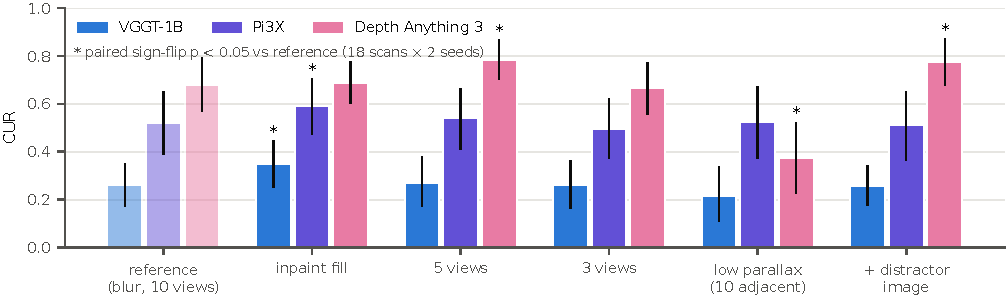
\includegraphics[width=0.92\textwidth]{fig6_stress}
\caption{\textbf{Stress tests.} \cur{} under each stress condition against the reference, with intervals. View count does nothing for VGGT and Pi3X; the inpainted fill raises leakage; DA3 alone reacts to parallax and to a distractor.}
\label{fig:stress}
\end{figure*}

\subsection{CO3Dv2: the ranking changes}
\label{sec:co3d}

\begin{table*}[t]
\centering
\caption{\textbf{CO3Dv2, five models, full configuration.} 18 scenes $\times$ 5 seeds $\times$ 2 radii $\times$ 3 fills, pooled over radii; mean [95\% CI over scenes]. Runs P2-co3d and P2-co3d-b.}
\label{tab:co3d}
\footnotesize
\setlength{\tabcolsep}{3pt}
\resizebox{\textwidth}{!}{\begin{tabular}{llccccccc}
\toprule
model & fill & \auroc & \cur & \curerr & $\absrel_S$ & $\absrel_U$ & $\absrel_U$ ctrl & conf ratio \\
\midrule
VGGT-1B & gray  & \ci{0.747}{0.692}{0.802} & \ci{0.565}{0.453}{0.677} & 0.029 & 0.029 & 0.031 & 0.027 & 0.634 \\
VGGT-1B & blur  & \ci{0.772}{0.717}{0.825} & \ci{0.534}{0.416}{0.652} & 0.034 & 0.029 & 0.031 & 0.027 & 0.603 \\
VGGT-1B & noise & \ci{0.590}{0.517}{0.656} & \ci{0.767}{0.693}{0.839} & 0.029 & 0.029 & 0.029 & 0.027 & 0.805 \\
Pi3 & gray  & \ci{0.930}{0.894}{0.958} & \ci{0.196}{0.118}{0.283} & 0.002 & 0.015 & 0.016 & 0.013 & 0.351 \\
Pi3 & blur  & \ci{0.903}{0.860}{0.939} & \ci{0.251}{0.170}{0.334} & 0.002 & 0.015 & 0.016 & 0.013 & 0.389 \\
Pi3 & noise & \ci{0.880}{0.813}{0.929} & \ci{0.293}{0.193}{0.405} & 0.002 & 0.015 & 0.015 & 0.013 & 0.472 \\
Pi3X & gray  & \ci{0.863}{0.825}{0.899} & \ci{0.329}{0.248}{0.408} & 0.001 & 0.017 & 0.022 & 0.014 & 0.749 \\
Pi3X & blur  & \ci{0.720}{0.661}{0.777} & \ci{0.584}{0.500}{0.668} & 0.002 & 0.017 & 0.018 & 0.014 & 0.877 \\
Pi3X & noise & \ci{0.743}{0.680}{0.798} & \ci{0.556}{0.462}{0.650} & 0.001 & 0.017 & 0.019 & 0.014 & 0.867 \\
MapAnything & gray  & \ci{0.609}{0.554}{0.665} & \ci{0.786}{0.721}{0.849} & 0.004 & 0.041 & 0.029 & 0.034 & 0.632 \\
MapAnything & blur  & \ci{0.575}{0.514}{0.637} & \ci{0.801}{0.735}{0.863} & 0.008 & 0.042 & 0.028 & 0.034 & 0.674 \\
MapAnything & noise & \ci{0.578}{0.524}{0.631} & \ci{0.819}{0.765}{0.870} & 0.007 & 0.041 & 0.033 & 0.034 & 0.690 \\
Depth Anything 3 & gray  & \ci{0.619}{0.560}{0.674} & \ci{0.816}{0.751}{0.877} & 0.001 & 0.019 & 0.015 & 0.014 & 0.874 \\
Depth Anything 3 & blur  & \ci{0.622}{0.574}{0.668} & \ci{0.813}{0.748}{0.872} & 0.001 & 0.018 & 0.015 & 0.014 & 0.853 \\
Depth Anything 3 & noise & \ci{0.618}{0.553}{0.679} & \ci{0.780}{0.702}{0.854} & 0.000 & 0.019 & 0.016 & 0.014 & 0.901 \\
\bottomrule
\end{tabular}}
\end{table*}

\begin{figure*}[t]
\centering
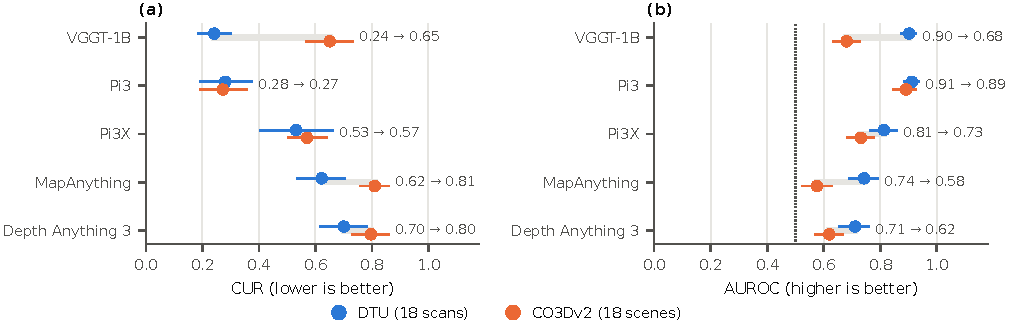
\includegraphics[width=0.92\textwidth]{fig4_dtu_vs_co3d}
\caption{\textbf{Lab rig versus phone captures.} Pooled blur-and-noise \cur{} and \auroc{} per model on DTU and CO3Dv2 with 95\% intervals. Pi3 is the only model whose numbers transfer; VGGT, MapAnything and DA3 leak markedly more on CO3Dv2.}
\label{fig:dtuco3d}
\end{figure*}

Table~\ref{tab:co3d} and Figure~\ref{fig:dtuco3d} repeat the full protocol on CO3Dv2 phone captures, with every threshold frozen from DTU. Pooled over blur and noise, \cur{} is 0.272 for Pi3, 0.570 for Pi3X, 0.651 for VGGT, 0.797 for DA3 and 0.810 for MapAnything; \auroc{} is 0.891, 0.732, 0.681, 0.620 and 0.576.

The ranking changes. Pi3 is the only model whose behaviour transfers from the lab rig to phone video (\cur{} 0.27 on both). VGGT, joint best on DTU, leaks 65\% of unsupported pixels on CO3Dv2, $2.7\times$ its DTU value, and under a noise fill its confidence is almost blind to non-observation (\auroc{} 0.59). MapAnything and DA3 let about four in five unsupported pixels through. After Holm correction, Pi3 leaks less than every other model ($p=0.0005$ each); Pi3X leaks less than MapAnything and DA3 ($p=0.0005$); VGGT leaks less than MapAnything ($p=0.010$) and DA3 ($p=0.0005$); VGGT versus Pi3X ($p=0.23$) and MapAnything versus DA3 ($p=0.73$) are not separated. Across datasets, the intervals of VGGT, MapAnything and DA3 do not overlap; those of Pi3 and Pi3X do.

\paragraph{Imagination is accurate here too.}
$\absrel_U$ is within 0.005 of $\absrel_S$ for every model, so \curerr{} stays below 0.04, and MapAnything's confident-and-wrong behaviour from DTU does not appear ($\absrel_S$ 0.041, \curerr{} 0.007). These are everyday objects with strong shape priors, and the models complete them well. The failure is, once more, that the completion is reported with the confidence of an observation. We had expected \cur{} and \curerr{} to separate on less predictable scenes; on CO3Dv2 they did not, and we leave the prediction standing for the heritage data.

\paragraph{Fill effects differ from DTU.}
On DTU every fill raised \cur{} over gray for VGGT, Pi3 and Pi3X. On CO3Dv2 noise raises VGGT's \cur{} by 0.20 ($p=0.00005$) but blur does not ($p=0.30$); Pi3X reacts to both ($+0.26$, $+0.23$); Pi3 reacts weakly ($+0.06$, $+0.10$, $p=0.007$ and $0.017$); MapAnything and DA3 do not react to the fill at all ($p$ from 0.06 to 0.91). A confidence that does not change when the patch changes is not reading the patch.

\paragraph{Per-scene view.}
Figure~\ref{fig:perscene} (supplementary) shows that the leak is not driven by a few scenes. Removing the one scene that missed the mask-transfer guard moves every pooled number by at most 0.013.


\subsection{Cheap detectors do not help}
\label{sec:cheap}

\begin{figure*}[t]
\centering
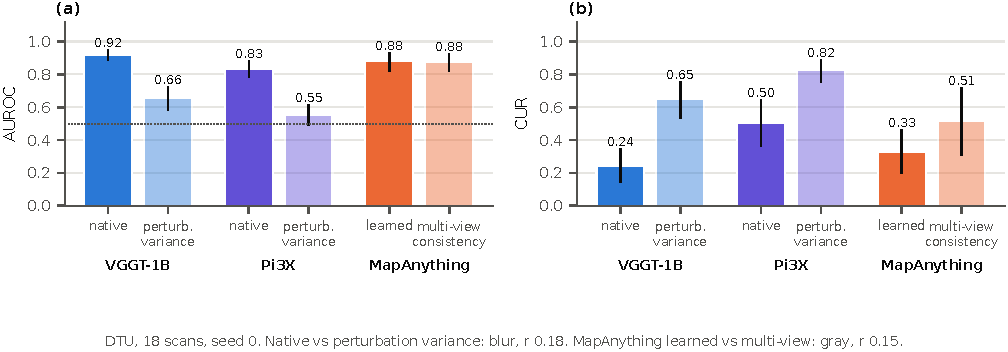
\includegraphics[width=0.92\textwidth]{fig8_cheap_detectors}
\caption{\textbf{Two training-free detectors against native confidence.} Perturbation variance (ReVar3R style, $K=4$ photometric perturbations, median-scale alignment) on VGGT and Pi3X, and MapAnything's multi-view consistency confidence against its learned confidence. Both are worse than the native signal on \auroc{} and \cur.}
\label{fig:cheap}
\end{figure*}

Two obvious alternatives are shown in Figure~\ref{fig:cheap} and Table~\ref{tab:detectors}. Variance over $K=4$ photometrically perturbed runs, aligned per sample by median scale, is much worse than native confidence on both backbones (VGGT \auroc{} 0.655 against 0.919, \cur{} 0.647 against 0.241; Pi3X 0.551 against 0.832, 0.824 against 0.502; paired $p\le0.00065$ in all four tests) while costing four forwards. The imagined geometry is stable under input perturbation, so sample variance is nearly the same on supported and unsupported pixels. This is the failure ReVar3R's authors describe as stable systematic bias, and it is why we draw disagreement from a generative head rather than from the input. MapAnything's multi-view consistency confidence leaks more than its learned confidence (\cur{} 0.51 against 0.34 in the smoke configuration). A fuller perturbation baseline (geometric augmentations, $K=8$, similarity alignment) is a required ablation before anyone should call the whole family insufficient; it is pending.

%------------------------------------------------------------------------
\section{Method: observe, imagine, abstain}
\label{sec:method}

\begin{figure*}[t]
\centering
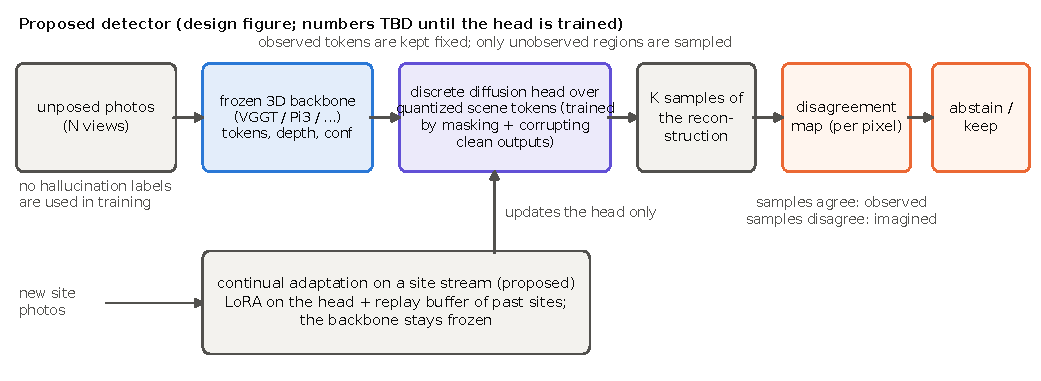
\includegraphics[width=0.8\textwidth]{fig9_method}
\caption{\textbf{Proposed method.} A frozen 3D backbone supplies geometry and tokens; frozen language-aligned features are concatenated at the same grid. A finite scalar quantizer turns geometry into discrete tokens, and a uniform-state discrete diffusion head, trained by masking 3D-consistent regions of clean backbone output and recovering their tokens, draws $K$ samples at test time. Agreement across samples and with the backbone marks \emph{observed}; agreement among samples but not with any observation marks \emph{imagined}; the remainder \emph{abstains}. Low-rank adapters with a replay buffer adapt the head to new sites. This figure specifies the design; its results are pending.}
\label{fig:method}
\end{figure*}

The benchmark says that native confidence does not know what the model has seen. Rather than suppress the prior, which is what makes these models useful, we want the model to say which of its outputs came from the prior. Figure~\ref{fig:method} shows the design.

\paragraph{Architecture.}
A frozen backbone (VGGT or Pi3X) provides per-pixel geometry and tokens. A frozen SigLIP2 ViT~\cite{siglip2} provides language-aligned features at the same grid, which later supports queries such as ``show only the observed part of the dome''. A finite scalar quantizer~\cite{fsq} turns backbone depth and local point outputs into discrete tokens. A discrete diffusion head of about 100M parameters with uniform-state corruption~\cite{ursa} denoises token grids conditioned on backbone and SigLIP2 features.

\paragraph{Training.}
Self-supervised. We mask random 3D-consistent regions of the clean backbone output (the same sphere mechanism as the benchmark, but on predictions rather than ground truth, so no labels are used), corrupt the tokens, and train the head to recover them. Hyperparameters are tuned on the DTU validation split and frozen before any other data is touched; the freeze date goes in the released log.

\paragraph{Inference.}
Draw $K$ samples. Per pixel: geometry is the per-sample median; disagreement is the token entropy across samples; the label is \emph{observed} if the backbone and all samples agree within a tolerance, \emph{imagined} if the samples agree with each other but not with any observation, and \emph{abstain} otherwise. The user sees three colours, not one confidence.

\paragraph{Compute.}
$K$ samples cost $K$ head passes on top of one backbone pass. We will report wall-clock and FLOPs and compare every baseline at equal compute, for instance perturbation variance with $K$ backbone passes.

\paragraph{Continual adaptation.}
A site stream (new monuments, new capture devices) is handled by low-rank adapters~\cite{lora} on the head with a small replay buffer of earlier sites. We will report new-site \auroc{} and \cur{} and old-site forgetting against naive fine-tuning and a frozen head.

%------------------------------------------------------------------------
\section{Experiments on the method}
\label{sec:exp}

\begin{table}[t]
\centering
\caption{\textbf{Detectors on DTU} (18 scans, seed 0, blur, radius 0.18; native rows from the same keys of the full run). Rows marked pending will be filled only from logged runs.}
\label{tab:detectors}
\footnotesize
\setlength{\tabcolsep}{3pt}
\resizebox{\columnwidth}{!}{\begin{tabular}{llccc}
\toprule
backbone & detector & fwd & \auroc & \cur \\
\midrule
VGGT-1B & native confidence & 1 & \ci{0.919}{0.890}{0.946} & \ci{0.241}{0.148}{0.343} \\
VGGT-1B & perturbation var., $K{=}4$ & 4 & \ci{0.655}{0.586}{0.724} & \ci{0.647}{0.536}{0.752} \\
VGGT-1B & reprojection consistency & 1 & \tbd{P3-reproj} & \\
VGGT-1B & $K$-sample disagreement (ours) & $1{+}K$ & \tbd{P3-main} & \\
Pi3X & native confidence & 1 & \ci{0.832}{0.782}{0.879} & \ci{0.502}{0.362}{0.642} \\
Pi3X & perturbation var., $K{=}4$ & 4 & \ci{0.551}{0.492}{0.609} & \ci{0.824}{0.753}{0.886} \\
Pi3X & $K$-sample disagreement (ours) & $1{+}K$ & \tbd{P3-main} & \\
\bottomrule
\end{tabular}}
\end{table}

\paragraph{What is measured and what is pending.}
Table~\ref{tab:detectors} holds the rows that exist. The pre-registered pass condition for the method is that $K$-sample disagreement beats native confidence on \auroc{} and \cur{} with a paired sign-flip $p<0.05$ over scans at equal compute; if it fails, this paper is a benchmark paper with the best training-free detector, and we will say so. The ablation grid ($K\in\{1,2,4,8,16\}$, fill, radius, backbone, with and without SigLIP2), the continual-adaptation stream and the heritage figure are \tbd{P3-abl, P4-cont, P4-heritage}. VGGT-Omega is gated and will be added when access is granted.

\paragraph{Fill ablation on the benchmark.}
Figure~\ref{fig:fills} (supplementary) collects the fill effects across both datasets, including the inpainted fill on DTU. It is the single figure we would point a sceptical reviewer to: the leak is largest when the patch is least visible.


%------------------------------------------------------------------------
\section{Limitations}
\label{sec:limits}

Static scenes only. The benchmark labels are a proxy for real occlusion: a real unobserved region is not surrounded by a filled patch, and the stress tests bound but do not remove that gap. Ground truth on CO3Dv2 is COLMAP depth with 1 to 3\% noise, so \absrel{} values below about 0.03 should be read as equal. DTU hides a region of a lab object; CO3Dv2 hides a region of a single everyday object; neither contains the long-range structure of a building. The method costs $K$ extra head passes at test time, and its results are pending. All findings depend on the released checkpoints and may change with newer ones.

%------------------------------------------------------------------------
\section{Conclusion}
\label{sec:conclusion}

We asked a simple question of five 3D foundation models: when you have not seen a surface, do you say so? The answer, measured on two datasets with free labels, is mostly no. Between a quarter and four fifths of the geometry these models invent passes a confidence filter tuned to keep 90\% of what they observed, the leak grows when the occluder looks natural, it does not shrink when fewer views are given, and the cheapest fix makes it worse. We think the right response is not to stop the models from imagining but to make them say when they do, and we have laid out a method and a pre-registered test for it. The benchmark, the code, and the complete run log, including the runs that failed, will be released.

\paragraph{Reproducibility.}
Every number in this paper maps to a CSV and a configuration file in the released log; the benchmark code is 700 lines of Python with no training; all model runs fit on a single 16 GB GPU in about eight hours total.

{\small
\bibliographystyle{ieeenat_fullname}
\bibliography{refs}
}


\clearpage
\onecolumn
\section*{Supplementary material}
\begin{figure}[h]
\centering
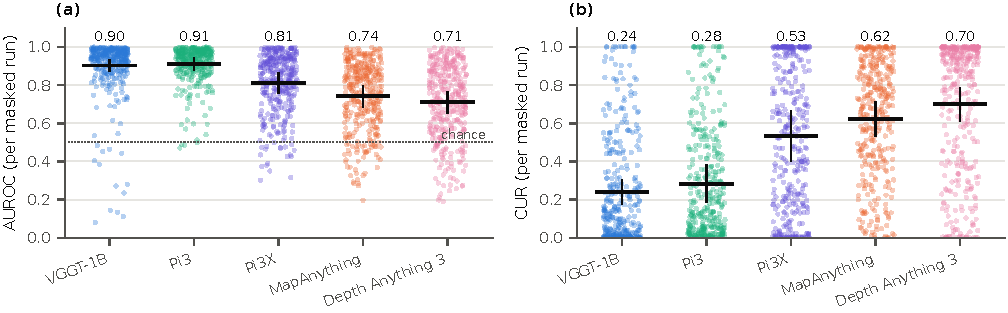
\includegraphics[width=0.95\textwidth]{fig3_metrics}
\caption{\textbf{Per-run spread on DTU.} \auroc{} and \cur{} for every (scan, seed, radius) run under blur and noise fills, with pooled means and intervals. The spread across scans is wide for every model; the intervals in the main tables come from resampling scans.}
\label{fig:metrics}
\end{figure}
\begin{figure}[h]
\centering
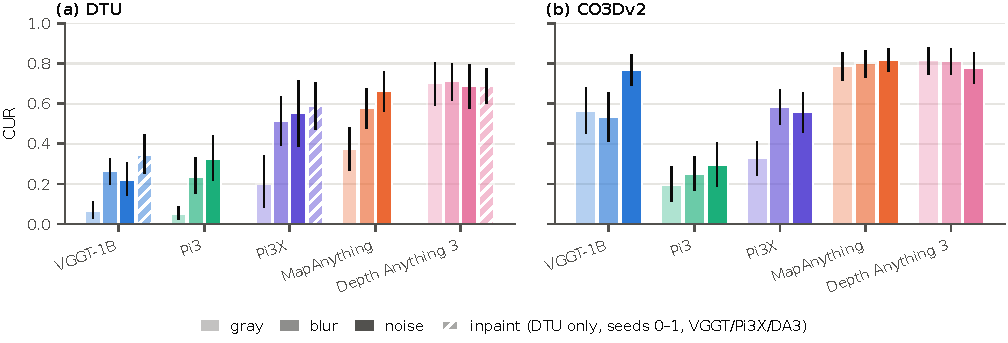
\includegraphics[width=0.95\textwidth]{fig5_fills}
\caption{\textbf{Fill ablation.} \cur{} per model and fill on DTU and CO3Dv2 (five seeds) and for the inpainted fill on DTU (two seeds, three models). A visible gray patch gives the lowest leakage; natural-statistics and inpainted fills give more.}
\label{fig:fills}
\end{figure}
\begin{figure}[h]
\centering
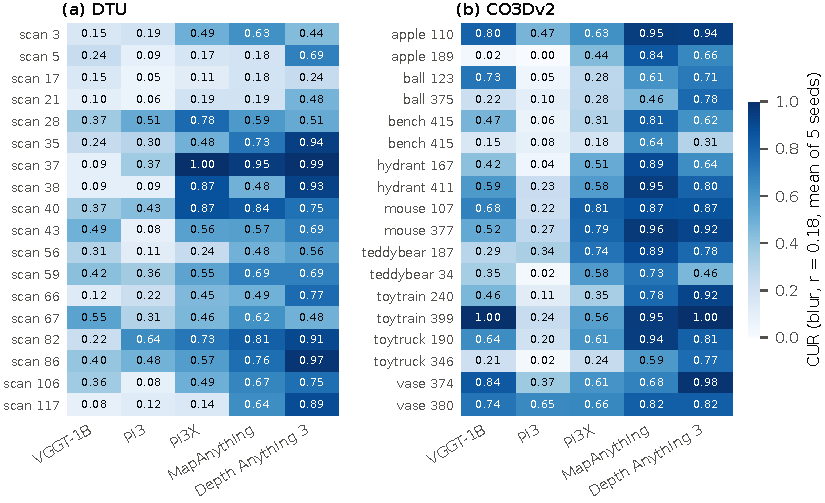
\includegraphics[width=0.95\textwidth]{fig7_perscene}
\caption{\textbf{Per-scene \cur{}} (blur fill, radius 0.18, mean over seeds) for every model on DTU scans and CO3Dv2 scenes. Rows are scenes, columns are models.}
\label{fig:perscene}
\end{figure}

\paragraph{Run registry.} Every table cell maps to a run id (P1-full, P2-full, P2-stress, P2-co3d, P2-co3d-b, P3-pv-smoke, P2-smoke-b) whose CSV, configuration JSON and kernel log are released with the code, together with the dated log of every failed run and every correction.

\end{document}
